\documentclass[12pt, a4paper]{article}
\usepackage[utf8]{inputenc}
\usepackage{hyperref}
\usepackage{graphicx}
\usepackage{enumitem}
\usepackage{upquote} 
\graphicspath{{./images/}}
\usepackage{tikz}
\usetikzlibrary{babel}
\usetikzlibrary{positioning, calc}
%%%%%%%%%%%%%%%
\title{my Accounting}
\author{Manuel Escriche Vicente}
\begin{document}
\maketitle
\begin{abstract}

\end{abstract}
\tableofcontents
\newpage

\section{Setup python environment}
Get a list of python installation:
\begin{verbatim}
>> type -a python
python is /Users/MANEV/.pyenv/shims/python
python is /usr/bin/python
\end{verbatim}
From this list, the first one is used:
\begin{verbatim}
>> which python
/Users/MANEV/.pyenv/shims/python
\end{verbatim}
Check what version of python is in use:
\begin{verbatim}
>> python -V
Python 3.8.6
\end{verbatim}
Check available versions
\begin{verbatim}
>> pyenv versions
  system
  3.6.1
* 3.8.6 (set by /Users/MANEV/.pyenv/version)
  3.9.16
\end{verbatim}
Set proper version in working folder.  
\begin{verbatim}
 >> pyenv local 3.9.16
 >> python -V 
 Python 3.9.16
 \end{verbatim}
 Install pipenv to setup our virtual python environment. Notice pipenv doesn't get the version established by pyenv local previously, but the global one. Therefore, you have to care to set it up again in next steps.
 \begin{verbatim}
 >> pip install pipenv
 >> pipenv install --python 3.9.16
 >> pipenv shell
 \end{verbatim}
 In case you have to remove your virtual environment 
 \begin{verbatim}
 >> pipenv --rm
 \end{verbatim}
 Install sqlalchemy
 \begin{verbatim}
 >> pipenv install sqlalchemy
 \end{verbatim}
 Now you're ready to configure the application for any user.
 
 %and, finally, execute the program
 %\begin{verbatim}
 %>> python myAccounting.py <user>
 %\end{verbatim} 
 
 \section{Configuration and administration }
 There are four  tools available for users configuration and for fixing emerging issues in the application:
 
 \begin{description}
 \item[config\_user.py] used to create the user's folder, and to copy the generic profile chosen into the specific \verb!<user>_profile.json!.
   The user profile file declares what accounts are used in your accounting,  and  how to build your income and balance reports.  
 \item[db\_tool.py] used to create user's data base, and populate it with the accounts.json file, and other useful utilities.
  \item[remake.py] used to rebuild the user data base and their year closing and opening seats consistently over the years.It is useful when having to modify the user first balance opening set, or when changes in the user profile file.
 \item[cmp\_files.py] used to compare two seats files. It is helpful to verify changes in the seat files after having saved them with \verb!db_tool save!
 \end{description}
 
 %%%%%%%%%%%%%%%%%%%%%%%
 \subsection{config\_user.py}
 Run \verb!>> python tools/config_user.py <user> create <profile>! \textbf{only one time} in order to create your \verb!<user>_profile.json! file, and its subsequent  operative application files at due place 
 \verb!\users\<user>\configfiles!:
\begin{figure}[h]
\centering
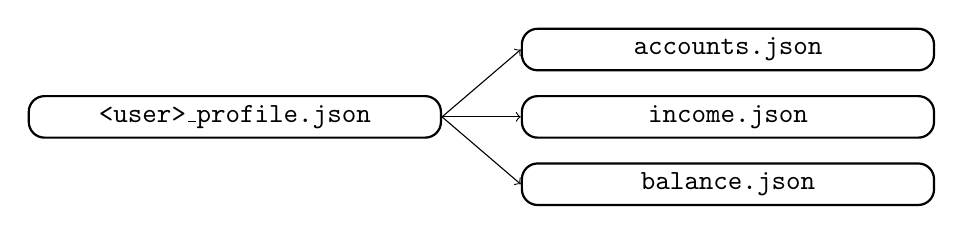
\begin{tikzpicture}[node distance = 3mm and 10mm,
file/.style= {rectangle, rounded corners= 2mm, align=center, thick, draw=black, text width= 50mm, font=\ttfamily} ]
\node (P) [file] {<user>\_profile.json};
\node (I) [file, right = of P] {income.json};
\node (A) [file, above =  of I] {accounts.json};
\node (B) [file, below = of I] {balance.json};
\path (P.east) edge[->] (I.west);
\path (P.east) edge[->] (A.west);
\path (P.east) edge[->] (B.west);
\end{tikzpicture}
 \end{figure}
  
Thereafter, any modification by hand in your \verb!<user>_profile.json! file, requires you  to run \verb!>> python tools/config_user.py <user> refresh! to regenerate consistently the application files; and depending on the changed content additional actions may be required. 
 
 \paragraph{Commands}
 \begin{verbatim}
 >> python tools/config_user.py <user> create <profile> 
 >> python tools/config_user.py <user> refresh
 \end{verbatim}
 %%%%%%%%%%%%%%%%%%%%%%%
 \subsection{db\_tool.py}
 Before starting you have to use this tool to create and prepare the user database. 
 Execute the following sequence:
 \begin{enumerate}[wide, labelwidth=!, labelindent=0pt]
 \item \verb!db_tool.py <user> create! to create user database file
 \item \verb!db_tool.py <user> init! to create user database structure		
 \item \verb!db_tool.py <user> setup!	 to populate user database with accounts
 \item \verb!db_tool.py <user> query! to verify accounts creation
 \item \verb!db_tool.py <user> save! to save yearly seats stored in the data base into files named with the tag \textsf{app} like \verb!YEAR_app_seats.json!. It's helpful when having to evolve the data base accounts, in companion of the \verb!remake! tool
\end{enumerate}
\paragraph{Commands}
\begin{verbatim}
>> python tools/db_tool.py <user> create
>> python tools/db_tool.py <user> init
>> python tools/db_tool.py <user> setup
>> python tools/db_tool.py <user> query
>> python tools/db_tool.py <user> save -t new
>> python tools/db_tool.py <user> remove
\end{verbatim}

\subsection{remake.py}
It's an important tool that allows to \verb!remake! the user data base and its corresponding accounting yearly closing and opening seat files from the user profile, starting opening seat, and yearly seats file available.
It's helpful when having to update the \verb!<user>_opening_seat.json! file, which requires to work it out all data, or when having to modify the \verb!<user>_profile.json! file because new accounts have been created, or its code modified.
\paragraph{Commands}
\begin{verbatim}
>> python tools/remake.py <user>   
>> python tools/remake.py <user> -t     
>> python tools/remake.py <user> -t new  
\end{verbatim}
\subsection{cmp\_files.py} 
Tool useful to compare json transactions files; especifically, \verb!year_<tag>_seats.json! file against \verb!<year>_app_seats.json! file.
\paragraph{Commands}
\begin{verbatim}
>> python tools/cmp_files.py <user> <year>     #tag = <user>
>> python tools/cmp_files.py <user> <year> -t new
\end{verbatim}
%%%%%%%%%%%%%%
  \section{Edition}
  \verb!myAccounting.py! is the main operating app for your personal accounting. 
  Seats are edited on its user interface, however since most of the seats are downloaded from the bank account in excel sheets, a specific tool has been made available.
 \paragraph{excel.py} tool used to take bank accounts excel files to export their transactions into json format so that main program can load them. 
 
 \paragraph{Commands}
 \begin{verbatim}
>> python tools/excel.py <user>
>> python myAccounting.py <user>
\end{verbatim}

 \subsection{Conceptual Model}
 Yet simple, but important to bear in mind:
 
 Transactions\footnote{Seats} are held in Journals. BookEntries  in Ledgers, and Accounts in  the Accounts Book. In data base terms, Journals, Ledgers and Accounts book are tables.  
 
 Besides, a transaction references several book entries; and each book entry references an account.
 Therefore, a transaction is build by aggregating a number of  records in the data base.
 
 Each record holds an identifier that makes it unique. However, when it comes to accounts, besides its unique data base id, they also have a unique code, which we set up in the profile file, and propagates to the \verb!accounts.json! file, and from there to the \verb!accounts! table in the data base.
 
 \paragraph{The first seat} is created when starting our accounting. This first seat that holds our opening balance is saved in a file, and from here by using the main app loaded into the data base. 
  \begin{figure}[h]
 \centering
 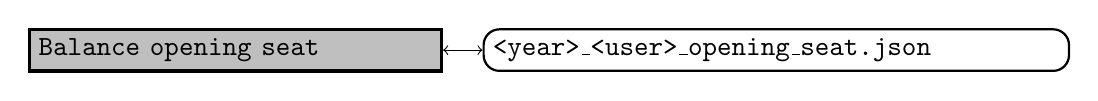
\begin{tikzpicture}[ node distance=5mm,
seat/.style={rectangle,draw=black, text width=50mm, font=\ttfamily},
file/.style={rectangle, rounded corners= 2mm, thick, draw=black, text width= 72mm, font=\ttfamily}]
\node (A) [seat, very thick, fill=lightgray] {Balance opening seat };
\node (B) [file, right = of A ] {<year>\_<user>\_opening\_seat.json};
\path (A) edge[<->] (B);
 \end{tikzpicture}
 \end{figure}

 \paragraph{The normal accounting year} has three mandatory seats, which are created by the main application upon user request, and are stored in different files. However, they must be loaded by the user to have an effect.
 \begin{figure}[h]
 \centering
 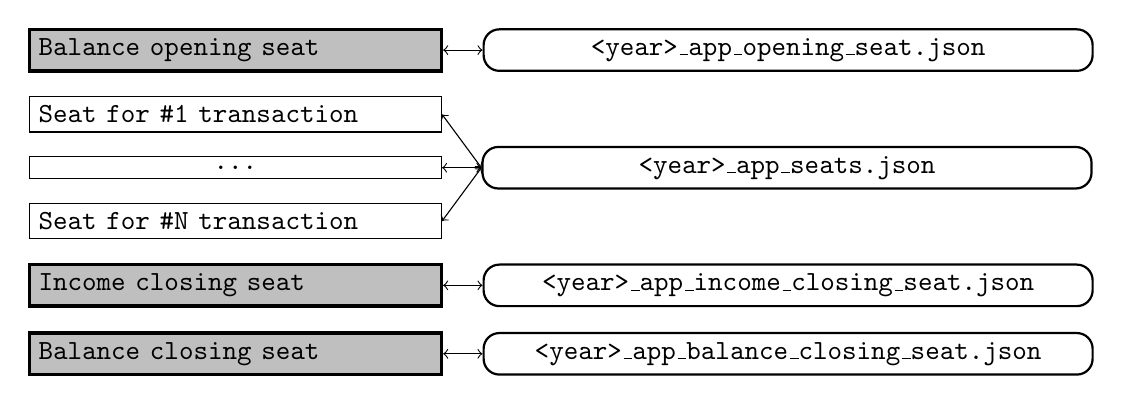
\begin{tikzpicture}[ node distance=3mm and 5mm,
seat/.style={rectangle,draw=black, text width=50mm, font=\ttfamily},
file/.style= {rectangle, rounded corners= 2mm, align=center, thick, draw=black, text width= 75mm, font=\ttfamily} ]
\node (A) [seat, very thick, fill=lightgray] {Balance opening seat};
\node (Af) [file, right = of A] {<year>\_app\_opening\_seat.json}; 
\node (B) [seat, below = of A] { Seat for \#1 transaction};
\node (C) [seat, below = of B, align=center] { \dots  };
\node (Cf) [file, right = of C] {<year>\_app\_seats.json}; 
\node (D) [seat, below = of C] { Seat for \#N transaction};
\node (E) [seat, very thick, fill=lightgray, below = of D] {Income closing seat};
\node (Ef) [file, right = of E] {<year>\_app\_income\_closing\_seat.json}; 
\node (F) [seat, very thick, fill=lightgray, below = of E] {Balance closing seat};
\node (Ff) [file, right = of F] {<year>\_app\_balance\_closing\_seat.json}; 

\path (A) edge[<->] (Af);
\path (E) edge[<->] (Ef);
\path (F) edge[<->] (Ff);

\path (B.east) edge[<->] (Cf.west);
\path (C) edge[<->] (Cf);
\path (D.east) edge[<->] (Cf.west);

 \end{tikzpicture}
 %\caption{Structure of  transactions in a year}
 \end{figure}

 \paragraph{Why are seats stored both in data base and files?}
 The application has been designed to store data both in the data base and in data files for safety reasons mainly. 
 Yet it isn't the only reason. As it is an accounting learning tool, it allows to you to evolve your accounting profile, or opening seat, and to \verb!remake! the data base and opening and closing seats consistently.
 

 %%%%%%%%%%%%%%%%%%%%%%%%
\section{Administration use cases}
\subsection{How to open the data base} \label{DB_open}
\begin{verbatim}
python
>>> import os, dbase
>>> root_dir = os.getcwd()
>>> username =  '<user>'
>>> user_dir = os.path.join(root_dir, 'users', username)
>>> dbase_file = os.path.join(user_dir, 'dbase', f'{username}_accounting.db')
>>> db_config =  {'sqlalchemy.url':f'sqlite+pysqlite:///{dbase_file}', 
	'sqlalchemy.echo':False}
>>> dbase.db_open(db_config)
>>> db = dbase.Session()
\end{verbatim}

\subsection{How to search an account  in the database} \label{DB_search_records}
Open data base as in \ref{DB_open}, then follow:
\begin{verbatim}
>>> from sqlalchemy import select
>>> from dbase import Account

>>> for item in db.query(Account): print(item)
>>> print(db.query(Account).filter_by(code=645).one())

>>> stmt = select(Account)
>>> for item in db.scalars(stmt): print(item)

>>> stmt = select(Account).where(Account.code.in_([64,641]))
>>> for item in db.scalars(stmt): print(item)

>>> stmt = select(Account).where(Account.code == 64)
>>> item = db.scalars(stmt).one()
>>> print(item)
\end{verbatim}

\subsection{How to search transactions}
Open the data base as in \ref{DB_open}, then follow:
\begin{verbatim}
>>> from sqlalchemy import select
>>> from dbase import Transaction, BookEntry

>>> stmt = select(Transaction)
>>> for item in db.scalars(stmt):print(item)

>>> stmt = select(Transaction).where(Transaction.id == 3902)
>>> item = db.scalars(stmt).one()
>>> print(item)
>>> for entry in item.entries: print(entry)

>>> stmt = select(BookEntry).join(Transaction).where(Transaction.id==3902)
>>> for item in db.scalars(stmt): print(item)

>>> items = db.query(BookEntry).join(Transaction).filter_by(id=3902)
>>> for item in items : print(item)

\end{verbatim}

\subsection{How to search  book entries in the data base} \label{DB_book_entries}
Open the data base as in \ref{DB_open}, then follow:
\begin{verbatim}
>>> from sqlalchemy import select
>>> from dbase import Account, Transaction, BookEntry

>>> for item in db.scalars(select(BookEntry)):print(item)
>>> for item in db.query(BookEntry): print(item)

>>> stmt = select(BookEntry).join(Account).where(Account.code==622)
>>> print(len(db.scalars(stmt).all()))
>>> for item in db.scalars(stmt): print(item)

>>> stmt = select(BookEntry).join(Transaction).where(Transaction.id==3882)
>>> for item in db.scalars(stmt): print(item)

\end{verbatim}

\subsection{How to modify an account description in the data base} \label{DB_account_description}
Open the data base as in \ref{DB_open}, then follow:
\begin{verbatim}
>>> from dbase import Account
>>> account = db.query(Account).filter_by(code = 613).one()
>>> account.name = "ExpP-Information/Formation"
>>> db.commit()
>>> item = db.get(dbase.Account, 23)
>>> print(item)
>>> quit()
>> python tools/db_tool.py <user> save 
>> python tools/remake.py <user>
\end{verbatim}

\subsection{How to modify a transaction description in the data base}
Open the data base as in \ref{DB_open}, then follow:
\begin{verbatim}
>>> from dbase import Transaction
>>> item = db.get(Transaction,1)
>>> item
Transaction(1 | 2015-11-15 | #entries=5 |  Opening statement)
>>> item.description
' Opening statement'
>>> item.description = 'Balance Opening Statement'
>>> db.commit()
>>> item = db.get(Transaction,1)
>>> item
Transaction(1 | 2015-11-15 | #entries=5 | Balance Opening Statement)
\end{verbatim}
 
 
 \subsection{How to create a new account for House Tax}  
 When a new account is created, only a new entry is created in the Account table. 
 So this action hasn't got a major impact in the data base. 
 However, it's important to declare it properly in the profile file, since income and balance reports depend on how those accounts' codes are included in their corresponding sections of the profile file. 
 
 Follow these steps:
 \begin{enumerate}
 \item Edit the \verb!<user>_profile.json! file
 \begin{enumerate}
 \item Open the file, which is located in the folder \verb!configfiles! with a text editor like \textsf{emacs}
 \item Add a new line, and  write the new entry in the \textbf{accounts} section\\ 
 	\verb!{"type":"DEBIT","content":"NOMINAL","code":"663","name":"Tax-House"}!
\item Skip the \textbf{balance} section, since the new account is  nominal
\item Search the \textbf{income} section, to add the new account's code under the \textbf{tax} concept:
	\verb! "tax": ["66", "661", "662", "663"], ! 
\item Save the file
\end{enumerate}
\item Run \verb!>> python tools/config_user.py <user> refresh! to regenerate the application files: \verb!accounts.json!, \verb!balance.json! and \verb!income.json! 
\item Run \verb!>> python tools/db_tool <user> setup! to  update data base account table with the records. 
 \end{enumerate}
 

\subsection{How to modify an account code}  
Let's take an example: on the profile we have the following entry:\\
\verb!{"type":"DEBIT","content":"NOMINAL","code":"621","name":"ExpH-Water"}!
where we want to transform the code \verb!621! to become \verb!6211!

Follow these steps:
\begin{enumerate}
\item Let's search book entries for account \verb!621! in the data base; by following steps in  \ref{DB_book_entries}, we find a number of records:  106 on this example. 
\item Let's make a backup of the data base before modifying it by running 
\verb!>> python tools/db_tool <user> backup!, that makes a backup copy.
\item Let's edit the \verb!<user>_profile.json! file
\begin{enumerate}
 \item Open the file, which is located in the folder \verb!configfiles! with a text editor.
 \item Modify the account's code in the line where it was declared. \\
 \verb!{"type":"DEBIT","content":"NOMINAL","code":"6211","name":"ExpH-Water"}!
 \item Skip the \textbf{balance} section, since the account is nominal
 \item Update the \textbf{income} section by modifying the account's code wherever it exists.\\
 \verb!"house": ["62", "6211", "622", "623", "624", "625", "626", "627"]!
 \item Save the file.
\end{enumerate}
\item Let's modify account code by following these steps:
 
Open the data base as in \ref{DB_open}, then follow:
\begin{verbatim}
>>> from dbase import Account
>>> account = db.query(Account).filter_by(code = 621).one()
>>> print(account)
Account(33 | Type.DEBIT | Content.NOMINAL | 621 | ExpH-Water | None )
>>> account.code = 6211
>>> db.commit()
>>> quit()
\end{verbatim}
\item Run \verb!>> python tools/db_tool.py <user> save! to save the database into files
\item Run \verb!>> python tools/config_user.py <user> refresh! to regenerate the application files: \verb!accounts.json!, \verb!balance.json! and \verb!income.json! 
\item Run \verb!>> python tools/remake.py <user>! to remake the data base
\end{enumerate}
 
\end{document}